\section{Regime Sinusoidale}
\begin{dfn}[Regime Sinusoidale]
	Condizione di funzionamento di un circuito a parametri concentrati in cui tutte le tensioni e le correnti sono rappresentabili tramite funzioni di tipo sinusoidale e isofrequenziali.
\end{dfn}
Sinusoide:
\[a(t) = A_Mcos(\omega t + \alpha)\]
Siano:
\begin{itemize}
	\item $A_M$ l'ampiezza dell'oscillazione (quanto vale il valore massimo rispetto allo 0);
	\item $\omega$ la pulsazione, in (rad/s). Vale $\omega = 2\pi f = \frac{2\pi}{T}$,  con $f$ frequenza, ossia numero di cicli al secondo e $T$ periodo, ossia tempo necessario per il compimento di un ciclo;
	\item $\alpha$ fase iniziale.
\end{itemize}
Proprietà delle funzioni sinusoidali.
\begin{itemize}
	\item È sempre possibile esprimere un seno come coseno e viceversa ($sin(x) = cos(x - \pi/2) \leftrightarrow cos(x) = sin(x+\pi/2)$), perciò si può parlare genericamente di funzioni sinusoidali, e trattarne una soltanto non causa perdita di generalità;
	\item Valor medio nullo.
	\[\overline a = \frac{1}{T} \int_{-T/2}{T/2} a(t)dt = 0\]
	\item \textsl{Valore efficace} (anche detto RMS, \textsl{root mean square}) $A$ in rapporto fisso con l'ampiezza
	\[A = \sqrt{\frac{1}{T} \int_{-T/2}^{T/2} a^2(t)dt} = \frac{A_M}{\sqrt{2}}\]
\end{itemize}
\subsection{Introduzione alla risoluzione di un circuito in regime sinusoidale}
Come abbiamo già visto per circuiti in corrente diretta, in generale la soluzione di un circuito può essere ottenuta applicando direttamente le Leggi di Kirchhoff:
\[
Soluzione \longleftrightarrow \begin{cases}
	LKT: f(v_k(t))\\
	LKC: f(i_k(t))\
	LC
\end{cases}\]
Nel caso di circuiti in regime sinusoidale, questo sistema presenta peculiare difficoltà tecniche dovute alla presenza delle funzioni sinusoidali stesse nelle LKT e LKC, e dalla presenza di leggi costitutive integro-differenziali.\\
Siccome le derivate e gli integrali delle sinusoidi sono a loro volta sinusoidi, sappiamo comunque che tutte le tensioni e correnti sono descritte da sinusoidi. Osserviamo anche che ogni sinusoide in un circuito in regime sinusoidale, nota la pulsazione, è descritta da due valori (ampiezza e fase iniziali). Proviamo dunque a operare con numeri complessi, descritti a loro volta dai valori di ampiezza e fase, per poi sviluppare un metodo generale che consenta la risoluzione di circuiti in regime sinusoidale con calcoli più semplici.\\
Il passaggio da sinusoidi a numeri complessi può essere effettuato in maniera semplice tramite la \textsl{Trasformata di Steinmetz}
\subsection{Trasformata di Steinmetz}
\begin{dfn}[Trasformata di Steinmetz]
	Operatore lineare che associa ad una sinusoide di pulsazione $\omega$ data un numero complesso in modo univoco.
	\[S[a(t)] = \frac{\sqrt{2}}{T} \int_{-T/2}^{T/2} a(t)e^{-j\omega t}dt = \frac{\sqrt{2}}{T} \frac{1}{2} A_M e^{j\alpha}T = Ae^{j\alpha} = \underline A\]
	Il numero complesso $\underline A$ è chiamato \textsl{fasore rappresentativo di a(t)}.
	Questa trasformata può essere intesa come un caso particolare della Trasformata di Fourier.
	\begin{figure}[H]
		\begin{tikzpicture}[
				thick,
				>=latex,
				scale=1.2,
				phasor/.style={->, line width=1.5pt, color=orange},
				function/.style={color=black, smooth},
				label_text/.style={font=\small\sffamily}
				]
				
				% --- Titolo ---
				\node[anchor=west] at (-1, 2.5) {\sffamily Interpretazione grafica della Trasformata di Steinmetz};
				
				% ==================================================================
				% --- RIGA 1: Caso alfa = 0 ---
				% ==================================================================
				
				% --- Grafico nel tempo (Sinistra) ---
				\begin{scope}
					% Etichette
					\node[above] at (0, 1.5) {$a(t)$, $\alpha=0$};
					
					% Assi
					\draw[->] (-0.5, 0) -- (4, 0) node[right] {$t$};
					\draw[->] (0, -1.2) -- (0, 1.5);
					
					% Linee tratteggiate per l'ampiezza
					\def\Am{0.8}
					\draw[dashed, thin] (0, \Am) -- (4, \Am);
					\draw[dashed, thin] (0, -\Am) -- (4, -\Am);
					
					% Funzione sinusoidale (Coseno con fase 0)
					\draw[function, domain=0:3.8, samples=100] plot (\x, {\Am * cos(deg(2.5*\x))});
					
					% Segno del valore iniziale
					\draw[thick] (0, \Am) -- (-0.2, \Am);
				\end{scope}
				
				% --- Freccia di trasformazione S[...] ---
				\begin{scope}[xshift=5cm, yshift=0cm]
					\node[above] at (0.8, 0) {S[$a(t)$]};
					\draw[->, line width=1pt] (0, 0) -- (1.5, 0);
				\end{scope}
				
				% --- Piano dei Fasori (Destra) ---
				\begin{scope}[xshift=8cm, yshift=0cm]
					% Assi Re/Im
					\draw[->] (-0.5, 0) -- (3.5, 0) node[right] {Re};
					\draw[->] (0, -1.2) -- (0, 2.5) node[above] {Im};
					\coordinate (O) at (0,0);
					
					% Fasore (su asse Reale)
					\draw[phasor] (O) -- (2.5, 0) node[right, below= 3 pt,black] {$\alpha=0$};
					
					% Etichetta Ampiezza A
					% Linea ondulata arancione per indicare la lunghezza
					\draw[orange, decorate, decoration={brace, amplitude=5pt}] (0.1, 0.2) -- (2.4, 0.2);
					\node[above, orange] at (1.25, 0.2) {$A=\frac{A_m}{\sqrt{2}}$};
				\end{scope}
				
				
				% ==================================================================
				% --- RIGA 2: Caso alfa > 0 ---
				% ==================================================================
				
				\begin{scope}[yshift=-4cm] % Sposta tutto giù di 4cm
					
					% --- Grafico nel tempo (Sinistra) ---
					\begin{scope}
						% Etichette
						\node[above] at (0, 1.5) {$\alpha>0$};
						
						% Assi
						\draw[->] (-1, 0) -- (4, 0) node[right] {$t$};
						\draw[->] (0, -1.2) -- (0, 1.5);
						
						% Linee tratteggiate
						\def\Am{0.8}
						\draw[dashed, thin] (-1, \Am) -- (4, \Am);
						\draw[dashed, thin] (-1, -\Am) -- (4, -\Am);
						
						% Funzione sinusoidale sfasata (Coseno traslato a sinistra)
						% Fase alfa/w = 0.4 circa nel disegno
						\def\shift{0.4} 
						\draw[function, domain=-0.8:3.8, samples=100] 
						plot (\x, {\Am * cos(deg(2.5*(\x + \shift)))});
						
						% Indicazione dello sfasamento alfa/w
						\draw[<->] (-\shift, -0.2) -- (0, -0.2);
						\node[below] at (-\shift/2, -0.2) {$\alpha/\omega$};
						
						% Segno della croce sul picco traslato
						\node[font=\small] at (-\shift, \Am) {$\times$};
					\end{scope}
					
					% --- Freccia di trasformazione S[...] ---
					\begin{scope}[xshift=5cm, yshift=0cm]
						\node[above] at (0.8, 0) {S[$a(t)$]};
						\draw[->, line width=1pt] (0, 0) -- (1.5, 0);
					\end{scope}
					
					% --- Piano dei Fasori (Destra) ---
					\begin{scope}[xshift=8cm, yshift=0cm]
						% Assi Re/Im
						\draw[->] (-0.5, 0) -- (3.5, 0) node[right] {Re};
						\draw[->] (0, -1.2) -- (0, 2.5) node[above] {Im};
						\coordinate (O) at (0,0);
						
						% Fasore (Sfasato di alfa)
						\def\alfaDeg{30} % Angolo di circa 30 gradi
						\draw[phasor] (O) -- (\alfaDeg:2.5) node[left = 150 pt, below=30 pt, black] {$\alpha$};
						
						% Etichetta Ampiezza A
						\coordinate (P) at (\alfaDeg:2.5);
						% Linea ondulata parallela al fasore
						\draw[orange, decorate, decoration={brace, amplitude=5pt}] 
						($(O)+(0.1, 0.2)$) -- ($(P)+(-0.1, 0.2)$);
						\node[above, orange, rotate=\alfaDeg] at ($(O)!0.5!(P) + (0, 0.3)$) {$A=A_m/\sqrt{2}$};
						
						% Arco per l'angolo alfa
						\draw[->] (1, 0) arc (0:\alfaDeg:1);
					\end{scope}
				\end{scope}
		\end{tikzpicture}
		\caption{Interpretazione grafica della Traformata di Steinmetz}
		\label{fig:steinmetzgraf}
	\end{figure}
\end{dfn}

\begin{dfn}[Antitrasformata di Steinmetz]
	Operatore lineare che associa ad un fasore la sinusoide di pulsazione $\omega$ nota.
	\[S^-1[\underline A] = \sqrt{2} Re(\underline A e^{j\omega t}) =  \sqrt{2} Re(Ae^{j (\omega t + \alpha)}) = A_M cos(\omega t + \alpha) = a(t)\]
	Il numero complesso $f(t) = \sqrt{2}\underline A e^{j\omega t}$ è chiamato \textsl{fasore rotante}. Si veda la \cref{fig:antisteinmetz} per un'interpretazione grafica dell'antitrasformata. L'esponenziale di modulo unitario con fase variabile nel tempo, con pulsazione $\omega$ consente il passaggio al dominio temporale
	\begin{figure}
		\centering
		\includegraphics[width=0.8\linewidth]{antisteinmetz}
		\caption{Interpretazione grafica dell'antitrasformata di Steinmetz}
		\label{fig:antisteinmetz}
	\end{figure}

\end{dfn}
Proprietà della Trasformata di Steinmetz e operazioni con i fasori:
\begin{itemize}
	\item linearità. Si dimostra facilmente dalla linearità della distributività della moltiplicazione tra numeri complessi e dalla linearità dell'operatore integrale.\\
	Se $c(t) = a(t) + b(t)$, $\underline C = \underline A + \underline B = [Re(A) + Re(B)] + j [Im(A) + Im(B)] = \sqrt{\underline A^2 + \underline B^2} e^{j(\alpha_A + \alpha_B)}$.
	\item Moltiplicazione per uno scalare $K \in \mathbb{R}$. $\underline C = K \underline A = K A e^{j\alpha} \iff \begin{cases}
		C=KA\\
		arg(\underline C) = \begin{cases}
			arg(\underline A), k>0\\
			arg(\underline A) + \pi , k<0
		\end{cases}
		\end{cases}$
	\item Moltiplicazione interna (Moltiplicazione per un numero complesse)$\underline Z \in \mathbb{C}= Z A e^{j\alpha_z + \alpha} \iff \begin{cases}
		C=ZA\\
		arg(\underline C) = arg (\underline Z) + arg(\underline A)
	\end{cases}$. 
	\item Trasformata della derivata. 
	\[S[\frac{d}{dt}a(t)] = S[-\omega A_M cos(\omega t + \alpha + \pi/2)] = \omega A_M/\sqrt{2} e^{j\alpha + \pi/2} = \omega \underline A e^{j\pi/2} = j\omega \underline A\]
	In questo modo, le operazioni di derivata temporale vengono ricondotte a operazioni algebriche.
	\[\frac{d}{dt} x(t) \longleftrightarrow j\omega \underline X\]
	\item Trasformata della funzione integrale.\\
	Analogamente,
	\[\int x(t)dt \longleftrightarrow \frac{1}{j\omega} \underline X\]
\end{itemize}
\subsection{Metodo Simbolico}
Possiamo dunque utilizzare trasformata e antitrasformata di Steinmetz per l'analisi di un circuito in regime sinusoidale evitando equazioni integro-differenziali, risolvendo quelle algebriche associate nel campo simbolico (complesso) associato, secondo il percorso in \cref{fig:schema_analisi}
\begin{figure}[H]
	\centering
	\begin{tikzpicture}[
		node distance = 3.5cm and 5cm,
		box/.style = {
			draw, rectangle, align=center, 
			minimum height=2cm, minimum width=4cm, thick
		},
		arrow/.style = {
			-{Stealth[length=3mm]}, line width=1pt
		}
		]
		
		% Box
		\node[box] (tl) {LKT, LKC \\ Leggi costitutive \\ $v(t), i(t)$};
		\node[box, below=of tl] (bl) {$v(t), i(t)$ \\ $\forall \text{ ramo}$};
		\node[box, right=of tl] (tr) {LKT, LKC \\ leggi cost. \\ $\underline{V}, \underline{I}$};
		\node[box, below=of tr] (br) {$\underline{V}, \underline{I}$ \\ $\forall \text{ ramo}$};
		
		%Frecce ed etichette
		\draw[arrow] (tl) -- node[above, midway] {$S[\dots]$} (tr);
		\draw[arrow] (br) -- node[above, midway] {$S^{-1}[\dots]$} (bl);
		\draw[arrow] (tr) -- node[right, midway, xshift=5mm, align=center, text=red] {Sistema di equazioni \\ ALGEBRICHE $\in \mathbb{C}$} (br);
		\draw[arrow] (tl) -- node[left, midway, xshift=-5mm, align=center] {Sistema di eq. \\ DIFFERENZIALI} (bl);
		
		% X rossa
		\coordinate (mid_left) at ($(tl)!.5!(bl)$);
		\draw[red, line width=1.7pt] (mid_left) +(-4mm, -4mm) -- +(4mm, 4mm);
		\draw[red, line width=1.7pt] (mid_left) +(-4mm, 4mm) -- +(4mm, -4mm);
		
		\end{tikzpicture}
		
		\caption{Schema del percorso di analisi nel dominio del tempo e della frequenza per circuiti in regime sinusoidale applicando il Metodo Simbolico, tramite la Trasformata di Steinmetz}
		\label{fig:schema_analisi}
	\end{figure}
\subsection{Leggi topologiche e costitutive in dominio simbolico}
\begin{legge}[Legge di Kirchhoff delle correnti]
	\[LKC: \sum_{k=1}^n i_k(t) = 0 \quad \xrightarrow{\text{S[...]}} \quad \sum_{k=1}^n \underline I_k(t) = 0 \]
\end{legge}

\begin{legge}[Legge di Kirchhoff delle tensioni]
	\[LKT: \sum_{k=1}^m v_k(t) = 0 \quad \xrightarrow{\text{S[...]}} \quad \sum_{k=1}^n \underline V_k(t) = 0 \]
\end{legge}

\begin{legge}[Legge costitutiva del resistore lineare]
	\[\underline V = R \underline I\]
	Nel campo complesso, dunque, i fasori rappresentativi di corrente e tensione sono in fase (\cref{fig:R_fas}). Nel dominio temporale, saranno rappresentati da due sinusoidi in fase, con ampiezza, in generale, differente (\cref{fig:R_t}). 
	\begin{figure}[H]
		\centering
		
		% --- 1. GRAFICO A SINISTRA (DOMINIO DEL TEMPO - RESISTORE) ---
		\begin{subfigure}[b]{0.6\textwidth}
			\centering
			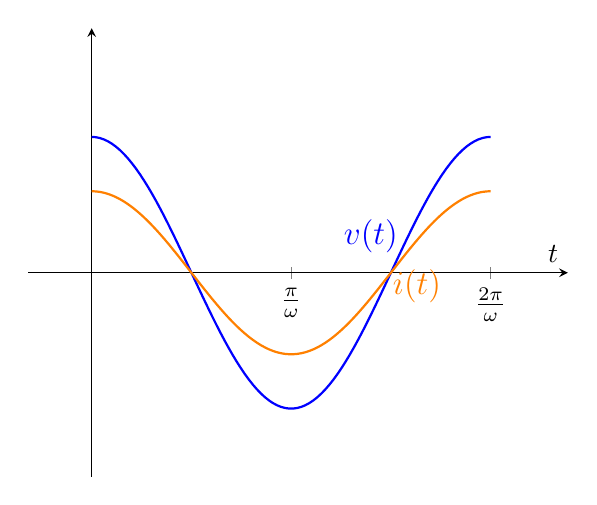
\begin{tikzpicture}
				\begin{axis}[
					axis lines=middle,
					xlabel=$t$,
					xtick = {0, 3.14159, 6.28318},
					xticklabels = {$0$, $\frac{\pi}{\omega}$, $\frac{2\pi}{\omega}$},
					ytick=\empty,
					xmin=-1,
					xmax=7.5,
					ymin=-1.5,
					ymax=1.8,
					clip=false
					]
					
					% --- Funzioni (IN FASE) ---
					% v(t) - sin(x) in BLU
					\addplot[
					blue, thick,
					domain=0:2*pi, 
					samples=100
					] {cos(deg(x))} 
					node[left, pos=0.8, font=\large] {$v(t)$};
					
					% i(t) - 0.6*sin(x) in ARANCIONE
					\addplot[
					orange, thick, 
					domain=0:2*pi, 
					samples=100
					] {0.6*cos(deg(x))} % <- MODIFICA: In fase, ampiezza minore
					node[right, below=7pt, pos=0.82, font=\large] {$i(t)$};
					
					% --- Dettagli (zeri) ---
					% Gli zeri ora si sovrappongono
					\node[blue, mark=x, scale=1.5] at (axis cs:0, 0) {};
					\node[blue, mark=x, scale=1.5] at (axis cs:pi, 0) {};
					\node[blue, mark=x, scale=1.5] at (axis cs:2*pi, 0) {};
					\node[orange, mark=x, scale=1.5] at (axis cs:0, 0) {};
					\node[orange, mark=x, scale=1.5] at (axis cs:pi, 0) {};
					\node[orange, mark=x, scale=1.5] at (axis cs:2*pi, 0) {};
				\end{axis}
			\end{tikzpicture}
			\caption{Grafico nel dominio del tempo (Resistore).}
			\label{fig:R_t}
		\end{subfigure}%
		% --- 2. GRAFICO A DESTRA (FASORI - RESISTORE) ---
		\begin{subfigure}[b]{0.4\textwidth}
			\centering
			\begin{tikzpicture}[
				thick,
				vettore/.style={-{Stealth[length=3mm]}, line width=1.5pt}
				]
				
				% --- Assi ---
				\draw[->] (-1,0) -- (4,0) node[below left] {Re};
				\draw[->] (0,-1) -- (0,4) node[below left] {Im};
				\coordinate (O) at (0,0);
				
				% --- Vettori (Fasori SOVRAPPOSTI) ---
				% Disegno prima il più lungo (V)
				\draw[vettore, blue] (O) -- (3.5,0) 
				node[above=2pt, blue] {$\underline{V}$};
				% Disegno dopo il più corto (I) per farlo stare sopra
				\draw[vettore, orange] (O) -- (2.5,0) 
				node[midway, above=2pt, orange] {$\underline{I}$};
				
				% --- Etichetta equazione (con colori) ---
				\node at (2.5, 1.5) { % Posizione aggiornata
					\textcolor{blue}{$\underline{V}$} = $R$ \textcolor{orange}{$\underline{I}$}
				};
				
			\end{tikzpicture}
			\caption{Diagramma fasoriale (Resistore).}
			\label{fig:R_fas}
		\end{subfigure}
		
		\caption{Confronto tra dominio del tempo e simbolico per un resistore.}
	\end{figure}
\end{legge}

\begin{legge}[Legge costitutiva del condensatore]
	\[i(t) = C \frac{dv(t)}{dt} \xrightarrow{\text{S[...]}} \begin{aligned}[t] 
		\underline I &= j \omega C \underline V\\
		\underline V &= -\frac{j}{\omega C} \underline I
	\end{aligned}
	\]
	Nel campo complesso, il fasore rappresentativo della corrente è sfasato di $\pi/2$ (in positivo) rispetto alla tensione (\cref{fig:cond_fas}). Nel dominio temporale, dunque, la corrente risulta "in anticipo" di una fase $\pi/2$ rispetto alla tensione (\cref{fig:cond_t}). Si dice anche che il fasore della corrente è \textsl{in quadratura in anticipo} rispetto alla tensione.
	Si ottiene la stessa conclusione considerando che $\frac{d}{dt} cos(t) = -sin(t)$.
	
	\begin{figure}[H]
		\centering
		
		% --- 1. GRAFICO A SINISTRA (DOMINIO DEL TEMPO) ---
		\begin{subfigure}[b]{0.6\textwidth}
			\centering
			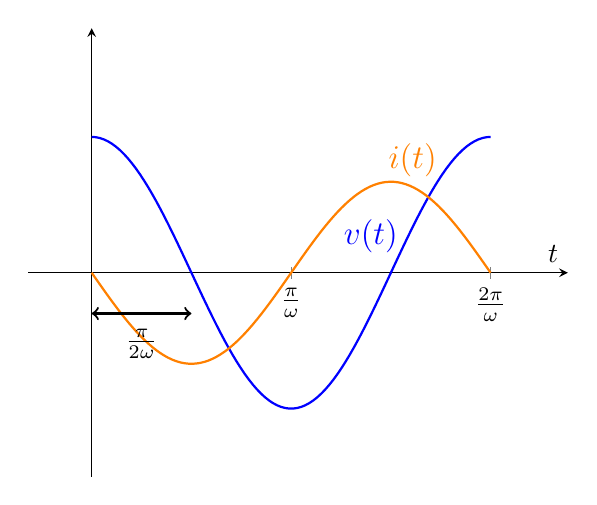
\begin{tikzpicture}
				\begin{axis}[
					axis lines=middle,
					xlabel=$t$,
					% --- MODIFICA: Ticks sull'asse x ---
					xtick = {0, 3.14159, 6.28318},
					xticklabels = {$0$, $\frac{\pi}{\omega}$, $\frac{2\pi}{\omega}$},
					% ---
					ytick=\empty,
					xmin=-1,
					xmax=7.5,
					ymin=-1.5,
					ymax=1.8,
					clip=false
					]
					
					% --- Funzioni ---
					% v(t) - sin(x) in BLU
					\addplot[
					blue, thick, % <- MODIFICA: Colore cambiato
					domain=0:2*pi, 
					samples=100
					] {cos(deg(x))} 
					node[left, pos=0.8, font=\large] {$v(t)$};
					
					% i(t) - cos(x) in arancione
					\addplot[
					orange, thick, 
					domain=0:2*pi, 
					samples=100
					] {-0.67*sin(deg(x))} 
					node[above, pos=0.8, font=\large] {$i(t)$};
					
					% --- Dettagli (zeri) ---
					% Segni 'x' per gli zeri
					\node[blue, mark=x, scale=1.5] at (axis cs:0, 0) {};
					\node[blue, mark=x, scale=1.5] at (axis cs:pi, 0) {};
					\node[blue, mark=x, scale=1.5] at (axis cs:2*pi, 0) {};
					\node[orange, mark=x, scale=1.5] at (axis cs:pi/2, 0) {};
					\node[orange, mark=x, scale=1.5] at (axis cs:1.5*pi, 0) {};
					
					% --- Frecce sui picchi rimosse ---
					
					% Freccia e etichetta fase
					\draw[<->, thick] 
					(axis cs:0, -0.3) -- (axis cs:{pi/2}, -0.3) 
					node[midway, below=2pt] {$\frac{\pi}{2\omega}$};
				\end{axis}
			\end{tikzpicture}
			\caption{Grafico nel dominio del tempo.}
			\label{fig:cond_t}
		\end{subfigure}%
		% --- 2. GRAFICO A DESTRA (FASORI) ---
		\begin{subfigure}[b]{0.4\textwidth}
			\centering
			\begin{tikzpicture}[
				thick,
				vettore/.style={-{Stealth[length=3mm]}, line width=1.5pt}
				]
				
				% --- Assi ---
				\draw[->] (-1,0) -- (4,0) node[below left] {Re};
				\draw[->] (0,-1) -- (0,4) node[below left] {Im};
				\coordinate (O) at (0,0);
				
				% --- Vettori (Fasori) ---
				% Fasore V in BLU
				\draw[vettore, blue] (O) -- (3,0) 
				node[midway, below=2pt, blue] {$\underline{V}$};
				% Fasore I in ARANCIONE
				\draw[vettore, orange] (O) -- (0,2) 
				node[midway, left=2pt, orange] {$\underline{I}$};
				
				% --- Etichetta equazione (con colori) ---
				\node at (2.5, 2.5) {
					\textcolor{orange}{$\underline{I}$} = $j\omega C$ \textcolor{blue}{$\underline{V}$}
				};
				
				% --- Angolo retto ---
				\coordinate (A) at (0.4, 0);
				\coordinate (B) at (0, 0.4);
				\draw (A) -- (0.4, 0.4) -- (B);
				
			\end{tikzpicture}
			\caption{Diagramma fasoriale.}
			\label{fig:cond_fas}
		\end{subfigure}
		\caption{Confronto tra dominio del tempo e dominio simbolico per un condensatore.}
	\end{figure}
\end{legge}

\begin{legge}[Legge costitutiva dell'induttore]
	\[v(t) = L \frac{di(t)}{dt} \xrightarrow{\text{S[...]}} \begin{aligned}[t] 
		\underline V &= j \omega L \underline I\\
		\underline I &= - j \frac{\underline V}{\omega L}
	\end{aligned}
	\]
	Nel campo complesso, il fasore rappresentativo della corrente è sfasato di $\pi/2$ (in negativo) rispetto alla tensione (\cref{fig:ind_fas}). Nel dominio temporale, dunque, la corrente risulta "in anticipo" di una fase $\pi/2$ rispetto alla tensione (\cref{fig:ind_t}). Si dice anche che il fasore della corrente è \textsl{in quadratura in ritardo} rispetto alla tensione.
	Si ottiene la stessa conclusione considerando che $\frac{d}{dt} cos(t) = -sin(t)$.
	
	\begin{figure}[H]
		\centering
		
		% --- 1. GRAFICO A SINISTRA (DOMINIO DEL TEMPO) ---
		\begin{subfigure}[b]{0.6\textwidth}
			\centering
			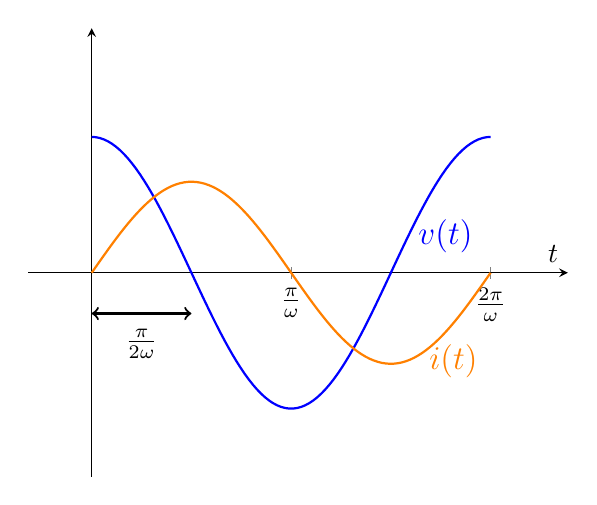
\begin{tikzpicture}
				\begin{axis}[
					axis lines=middle,
					xlabel=$t$,
					% --- MODIFICA: Ticks sull'asse x ---
					xtick = {0, 3.14159, 6.28318},
					xticklabels = {$0$, $\frac{\pi}{\omega}$, $\frac{2\pi}{\omega}$},
					% ---
					ytick=\empty,
					xmin=-1,
					xmax=7.5,
					ymin=-1.5,
					ymax=1.8,
					clip=false
					]
					
					% --- Funzioni ---
					% v(t) - sin(x) in BLU
					\addplot[
					blue, thick, % <- MODIFICA: Colore cambiato
					domain=0:2*pi, 
					samples=100
					] {cos(deg(x))} 
					node[right, pos=0.8, font=\large] {$v(t)$};
					
					% i(t) - cos(x) in arancione
					\addplot[
					orange, thick, 
					domain=0:2*pi, 
					samples=100
					] {0.67*sin(deg(x))} 
					node[right, below=4pt, pos=0.9, font=\large] {$i(t)$};
					
					% --- Dettagli (zeri) ---
					% Segni 'x' per gli zeri
					\node[blue, mark=x, scale=1.5] at (axis cs:0, 0) {};
					\node[blue, mark=x, scale=1.5] at (axis cs:pi, 0) {};
					\node[blue, mark=x, scale=1.5] at (axis cs:2*pi, 0) {};
					\node[orange, mark=x, scale=1.5] at (axis cs:pi/2, 0) {};
					\node[orange, mark=x, scale=1.5] at (axis cs:1.5*pi, 0) {};
					
					% --- Frecce sui picchi rimosse ---
					
					% Freccia e etichetta fase
					\draw[<->, thick] 
					(axis cs:0, -0.3) -- (axis cs:{pi/2}, -0.3) 
					node[midway, below=2pt] {$\frac{\pi}{2\omega}$};
				\end{axis}
			\end{tikzpicture}
			\caption{Grafico nel dominio del tempo.}
			\label{fig:ind_t}
		\end{subfigure}%
		% --- 2. GRAFICO A DESTRA (FASORI) ---
		\begin{subfigure}[b]{0.4\textwidth}
			\centering
			\begin{tikzpicture}[
				thick,
				vettore/.style={-{Stealth[length=3mm]}, line width=1.5pt}
				]
				
				% --- Assi ---
				\draw[->] (-1,0) -- (4,0) node[below left] {Re};
				\draw[->] (0,-1) -- (0,4) node[below left] {Im};
				\coordinate (O) at (0,0);
				
				% --- Vettori (Fasori) ---
				% Fasore V in BLU
				\draw[vettore, blue] (O) -- (3,0) 
				node[midway, below=2pt, blue] {$\underline{V}$};
				% Fasore I in ARANCIONE
				\draw[vettore, orange] (O) -- (0,-2) 
				node[midway, left=2pt, orange] {$\underline{I}$};
				
				% --- Etichetta equazione (con colori) ---
				\node at (2.5, 2.5) {
					\textcolor{orange}{$\underline{I}$} = $j\omega L$ \textcolor{orange}{$\underline{I}$}
				};
				
				% --- Angolo retto ---
				\coordinate (A) at (0.4, 0);
				\coordinate (B) at (0, 0.4);
				\draw (A) -- (0.4, 0.4) -- (B);
				
			\end{tikzpicture}
			\caption{Diagramma fasoriale.}
			\label{fig:ind_fas}
		\end{subfigure}
		\caption{Confronto tra dominio del tempo e dominio simbolico per un induttore.}
	\end{figure}
\end{legge}

\subsection{Legge di Ohm simbolica}
Osserviamo, dunque, che per i componenti descritti sopra, i fasori tensione e corrente sono sempre proporzionali, con costanti diverse (\cref{fig:impedenza}). Definiamo dunque l'\textsl{impedenza} come tale costante di proporzionalità. Questa grandezza ci sarà utile per formulare l'equivalente della Legge di Ohm in dominio simbolico. 
\begin{figure}[H]
	\centering
	\includegraphics[width=0.7\linewidth]{impedenza}
	\caption{}
	\label{fig:impedenza}
\end{figure}

\begin{dfn}[Impedenza]
	Definiamo \textsl{Impedenza} $\underline Z \in \mathbb{C}$
	\[\underline Z = \frac{\underline V}{\underline I}\]
	Essa rappresenta quanto il bipolo a cui è riferita si oppone al passaggio di una corrente alternata in regime sinusoidale.\\
	Chiamiamo \textsl{sfasamento} la quantità $\varphi = arg(\underline Z) = \alpha_V - \alpha_I$ e \textsl{reattanza} la parte immaginaria dell'impedenza, mentre notiamo che la parte reale dell'impedenza coincide con la resistenza del componente. La reattanza può assumere qualunque valore reale. La resistenza di un componente non è mai negativa, ma nell'analisi dei circuiti equivalenti che condurremo in seguito è possibile che emergano resistenze negative.
	\[\underline Z = \frac{V}{I}e^{j(\alpha_V - \alpha_I)} = Z cos(\varphi) + jZ sin(\varphi) = R + j X\]
	Seguendo il procedimento contrario,
	\[\begin{aligned}
		&Z = |\underline Z| = \sqrt{R^2 + X^2}\\
		&\varphi = \arg(\underline Z) = \begin{cases}
			atan(X/R), R>0\\
			atan(X/R) \pm \pi, R<0
		\end{cases}
	\end{aligned}\]
	
	Studiamo l'impedenza dei bipoli considerati.
	\begin{itemize}
		\item Per un resistore, \[
		\begin{aligned}
			&Z_R = R\\
			&\varphi_R = arg (\underline Z_R) = 0
		\end{aligned}\]
		Un bipolo di questo tipo, con reattanza nulla, è detto \textsl{ohmico};
		\item Per un condensatore, la resistenza è nulla. Si osservi che la reattanza è negativa.
		\[\underline Z_C = -\frac{j}{\omega C} =  X_C \iff 
		\begin{aligned}
			&Z_C = \frac{1}{\omega C}\\
			&\varphi_C = arg(\underline Z_C) = -\frac{\pi}{2}
		\end{aligned}\]
		\item Per un induttore, la resistenza è nulla. Si osservi che la (reattanza) è positiva
		\[\underline Z_L = j\omega L =  X_L \iff 
		\begin{aligned}
			&Z_L = \omega L\\
			&\varphi_L = arg(\underline Z_L) = \frac{\pi}{2}
		\end{aligned}\]
	\end{itemize}
\end{dfn}
\begin{dfn}[Ammettenza]
	Analogamente a come abbiamo introdotto la conduttanza come reciproco della resistenza, definiamo l'\textsl{Ammettenza}
	\[\underline Y = \frac{1}{\underline Z} = \frac{I}{V} e^{j (-\varphi)} = \frac{R}{R^2 + X^2} + j (-\frac{X}{R^2 + X^2})= G + jB\]
	dove $G$ è la conduttanza, e coincide con $1/R$ nel caso di un bipolo ohmico; e $B$ è detto \textsl{suscettanza} e in caso di bipolo induttivo o capacitivo $B=-1/X$.
\end{dfn}

\begin{legge}[Legge di Ohm simbolica]
	Con riferimento al bipolo generico in \cref{fig:ohmsimb} con la convenzione dell'utilizzatore, valgono le seguenti relazioni, che esprimono la Legge di Ohm in dominio simbolico:
	\[\underline V = \underline Z \underline I \quad \longleftrightarrow \quad v=Ri\]
	\[\underline I = \underline Y \underline V \quad \longleftrightarrow \quad i = Gv\]	
	\begin{figure}[H]
		\centering
		\includegraphics[width=0.5\linewidth]{ohm_simb}
		\caption{}
		\label{fig:ohmsimb}
	\end{figure}
\end{legge}

\begin{ex}
	Con riferimento al circuito in \cref{fig:circsimb}
	\begin{itemize}
		\item Trovare i fasori delle correnti in tutti i rami del circuito
		\item Determinare l'andamento temporale di $i_{g1}(t)$
	\end{itemize}
	\begin{figure}[H]
		\centering
		\includegraphics[width=0.7\linewidth]{circsimb}
		\caption{$R_1 = 1\ \Omega$, $R_2 = 2\ Omega$, $L=1\ mH$, $C= 1\ mF$, $V_{g1}= 12\sqrt{2} cos(\omega t + \pi/2)$ , $\omega = 2\pi f$, $f=10^3\ rad/s$ }
		\label{fig:circsimb}
	\end{figure}
	
	Soluzione. Come indicato nello schema in \cref{fig:schema_analisi}: 
	\begin{itemize}
		\item [1.]Circuito in dominio simbolico
		\item [2.]Trasformazione di Steinmetz delle leggi costitutive
		\item [3.]Soluzione di $\underline V, \underline I$
		\item [4.] Antitrasformazione di Steinmetz per ottenere $v(t), i(t)$.
	\end{itemize}
	
	Dunque, per la risoluzione dell'esercizio, si può scrivere il sistema:
	\[\begin{cases}
		\underline V_{g1} = S[V_{g1}] = 12 e^{j\pi/2} = j12\\
		\underline Z_{R1} = 1\\
		\underline Z_{R2} = 2\\
		\underline Z_L = j\omega L = j\\
		\underline Z_C = \frac{j}{\omega C} = -j\\		
	\end{cases}\]
	
	Osserviamo che le semplificazioni in serie e parallelo utilizzate per resistori, funzionano in maniera analoga per le impedenze:
	\[\begin{aligned}
		&\underline Z_{serie} = \sum_k \underline Z_k\\
		&\underline Z_{parallelo} = \frac{1}{\sum_k \frac{1}{\underline Z_k}}
	\end{aligned}\]
	Semplificando il nostro circuito, otteniamo:
	\[\begin{aligned}
		\begin{cases}
			\underline Z_{eq1} = Z_{R1} + \underline Z_L = 1+j\\
			\underline Z_{eq2} = \frac{\underline Z_C Z_{R2}}{\underline Z_C+ Z_{R2}} = 0,4 - j0,8\\
		\end{cases}\\
		\underline Z_{eq3} = \underline Z_{eq1} + \underline Z_{eq2} = 1,4 + j0,2\\
	\end{aligned}
	\]
	Risulta dunque:
	\[\underline I_{g1} = \frac{\underline V_{g1}}{\underline Z_{eq3}} = 1,2 + j 8,4\]
	Facendo riferimento al circuito originario,
	\[\begin{cases}
		\underline I_{R1} = \underline I_L = \underline I_{g1}\\
		\underline I_C = \underline I_{g1}\frac{Z_{R2}}{\underline Z_{R2} + \underline Z_C} = -2,4 + j 7,2\\
		\underline I_{R2} = \underline I_{g1} - \underline I_C = 3,6 + j 1,2
	\end{cases}\]
	E infine, considerando che
	\[\begin{cases}
		I_{g1} = \sqrt{Re(\underline I_{g1})^2 + Im(\underline I_{g1}^2)}= \sqrt{1,2^2 + 8,4^2} = 8,49\ A\\
		arg(\underline I_{g1}) = atan(8,4/1,2) = 1,43\ rad\\
	\end{cases}
	\]
	si ottiene:
	\[i_{g1}(t) = S^{-1}[\underline I_{g1}] = \sqrt{2} I_{g1} cos(\omega t + arg (\underline I_{g1})) =\sqrt{2} I_{g1} cos(\omega t + arg (\underline I_{g1})) =8,49\sqrt{2}  cos(2000\pi t + 1,43)\ A\]
\end{ex}
\subsection{Potenza in regime sinusoidale}
In generale, sappiamo che $p_A(t) = v(t) i(t)\quad (W)$.
In regime sinusoidale, tuttavia è possibile trovarne un'espressione più funzionale.
Consideriamo $\alpha_V = 0$ e $\alpha_I = -\varphi$, per semplificare i calcoli, senza perdita di generalità. Consideriamo una corrente in ritardo perché, generalmente, nelle applicazioni pratiche, la corrente è effettivamente in ritardo, perché i sistemi sono dominati da componente induttiva.\\
\[\begin{aligned}
	&v(t) = V_M cos(\omega t)\\
	&i(t) = I_M cos(\omega t - \varphi) = I_Mcos(\omega t)cos(\varphi) + I_M sin(\omega t)sin(varphi)=i_a(t) + i_r(t)
\end{aligned}\]
Chiamiamo il primo termine della corrente,  $i_a(t)$, in fase con la tensione, \textsl{corrente attiva}, mentre il secondo termine, $i_r(t)$, in quadratura con la tensione \textsl{corrente reattiva}.
\[p(t) = v(t)\cdot (i_a(t) + i_r(t) = v(t)i_a(t) + v(t)i_r(t)\]
Studiamo ora i due termini dell'espressione della potenza.

\begin{dfn}[Potenza istantanea attiva]
	Chiamiamo \textsl{potenza istantanea attiva} il termine:
	\[p_a(t) = v(t)i_a(t) = V_Mcos(\omega t)I_M cos(\omega t)cos(\varphi) = V_MI_Mcos^2(\omega t)cos(\varphi)=\frac{V_MI_M}{2}[1 + cos(2\omega t)]cos(\varphi)\]
	Da considerazioni analitiche, o dalla rappresentazione in \cref{fig:pot_att}, si osserva che:
	\begin{itemize}
		\item ha frequenza doppia rispetto a $v(t)$ e $i(t)$
		\item ha valore medio $\neq 0$
		\item è \textsl{unidirezionale} ($p_a(t) \geq 0 \quad \forall t$)
		\item $w(t) = \int p(t)dt \geq 0$ (ombreggiato in \cref{fig:pot_att}).
		\item essa è associata ai bipoli ohmici, o alla componente ohmica di bipoli non puri.
	\end{itemize}
	Per questo si conclude che la potenza istantanea attiva produce un lavoro "utile".
	
	\begin{figure}[H]
		\centering
		\begin{subfigure}[b]{0.8\textwidth}
			\centering
			\begin{tikzpicture}
				\begin{axis}[
					axis lines=middle,
					xlabel=$t$,
					% --- MODIFICA: Ticks sull'asse x ---
					xtick = {0, 3.14159, 6.28318},
					xticklabels = {$0$, $\frac{\pi}{\omega}$, $\frac{2\pi}{\omega}$},
					% ---
					ytick=\empty,
					xmin=-1,
					xmax=7.5,
					ymin=-1.5,
					ymax=2.0,
					clip=false
					]
					
					% --- Funzioni ---
					% v(t) - sin(x) in BLU
					\addplot[
					blue, thick, % <- MODIFICA: Colore cambiato
					domain=0:2*pi, 
					samples=100
					] {cos(deg(x))} 
					node[right, font=\large] {$v(t)$};
					
					% i(t) - cos(x) in arancione
					\addplot[
					orange, thick, 
					domain=0:2*pi, 
					samples=100
					] {0.67*cos(deg(x))} 
					node[right, font=\large] {$i_a(t)$};
					
					\addplot[
					magenta, thick, 
					domain=0:2*pi, 
					samples=100,
					name path=plotp,
					] {0.67*(1 + cos(deg(2*x)))*0.5} 
					node[above=3pt, pos= 0.5, font=\large] {$p_a(t)$};
					\path[name path=xaxis] (axis cs:0,0) -- (axis cs:2*pi,0);
					\addplot[
					pattern=north east lines,   % Stile tratteggio
					pattern color=magenta!60,      % Colore del tratteggio
					opacity=0.4                 % Leggera trasparenza
					] 
					fill between[
					of = plotp and xaxis,       % Riempie tra 'plot_v' e l'asse x
					soft clip={domain=0:2*pi}   % Solo nel dominio della funzione
					];
					
					% --- Dettagli (zeri) ---
					% Segni 'x' per gli zeri
					\node[blue, mark=x, scale=1.5] at (axis cs:0, 0) {};
					\node[blue, mark=x, scale=1.5] at (axis cs:pi, 0) {};
					\node[blue, mark=x, scale=1.5] at (axis cs:2*pi, 0) {};
					\node[orange, mark=x, scale=1.5] at (axis cs:pi/2, 0) {};
					\node[orange, mark=x, scale=1.5] at (axis cs:1.5*pi, 0) {};
					
				\end{axis}
			\end{tikzpicture}
		\end{subfigure}
		\caption{Possibile andamento della potenza istantanea attiva, per valori arbitrari di $V_M$, $I_M$ e $cos(\varphi)$. Si osservi che nel caso estremale in cui }
		\label{fig:pot_att}
	\end{figure}
\end{dfn}

\begin{dfn}[Potenza istantanea reattiva]
	Chiamiamo \textsl{potenza istantanea reattiva} il termine:
	\[p_r(t) = v(t)i_r(t) = V_Mcos(\omega t)I_M sin(\omega t)sin(\varphi) =\frac{V_MI_M}{2}sin(2\omega t)sin(\varphi)\]
	Da considerazioni analitiche, o dalla rappresentazione in \cref{fig:pot_reatt}, si osserva che:
	\begin{itemize}
		\item ha frequenza doppia rispetto a $v(t)$ e $i(t)$
		\item ha valore medio $= 0$
		\item è \textsl{bidirezionale} ($p_a(t) \gtrless 0$)
		\item $w(t) = \int_{-T/2}^{T/2} p(t)dt = 0$ (ombreggiato in \cref{fig:pot_reatt}).
		\item essa è associata ai bipoli reattivi, o alla componente reattiva di bipoli non puri.
	\end{itemize}
	Per questo si conclude che la potenza istantanea reattiva non produce lavoro utile (perché non produce lavoro netto).
	
	\begin{figure}[H]
		\centering
		\begin{subfigure}[b]{0.8\textwidth}
			\centering
			\begin{tikzpicture}
				\begin{axis}[
					axis lines=middle,
					xlabel=$t$,
					% --- MODIFICA: Ticks sull'asse x ---
					xtick = {0, 3.14159, 6.28318},
					xticklabels = {$0$, $\frac{\pi}{\omega}$, $\frac{2\pi}{\omega}$},
					% ---
					ytick=\empty,
					xmin=-1,
					xmax=7.5,
					ymin=-1.5,
					ymax=2.0,
					clip=false
					]
					
					% --- Funzioni ---
					% v(t) - sin(x) in BLU
					\addplot[
					blue, thick, % <- MODIFICA: Colore cambiato
					domain=0:2*pi, 
					samples=100
					] {cos(deg(x))} 
					node[right, font=\large] {$v(t)$};
					
					% i(t) - cos(x) in arancione
					\addplot[
					orange, thick, 
					domain=0:2*pi, 
					samples=100
					] {0.67*sin(deg(x))} 
					node[above, font=\large] {$i_a(t)$};
					
					\addplot[
					magenta, thick, 
					domain=0:2*pi, 
					samples=100,
					name path=plotp,
					] {0.67*sin(deg(2*x))*0.5} 
					node[above=3pt, pos= 0.7, font=\large] {$p_r(t)$};
					
					\path[name path=xaxis] (axis cs:0,0) -- (axis cs:2*pi,0);
					\addplot[
					pattern=north east lines,   % Stile tratteggio
					pattern color=magenta!60,      % Colore del tratteggio
					opacity=0.4                 % Leggera trasparenza
					] 
					fill between[
					of = plotp and xaxis,       % Riempie tra 'plot_v' e l'asse x
					soft clip={domain=0:2*pi}   % Solo nel dominio della funzione
					];
					% --- Dettagli (zeri) ---
					% Segni 'x' per gli zeri
					\node[blue, mark=x, scale=1.5] at (axis cs:0, 0) {};
					\node[blue, mark=x, scale=1.5] at (axis cs:pi, 0) {};
					\node[blue, mark=x, scale=1.5] at (axis cs:2*pi, 0) {};
					\node[orange, mark=x, scale=1.5] at (axis cs:pi/2, 0) {};
					\node[orange, mark=x, scale=1.5] at (axis cs:1.5*pi, 0) {};
					
				\end{axis}
			\end{tikzpicture}
		\end{subfigure}
		\caption{Possibile andamento della potenza istantanea reattiva, per valori arbitrari di $V_M$, $I_M$ e $cos(\varphi)$}
		\label{fig:pot_reatt}
	\end{figure}
\end{dfn}
Ricapitolando:
\begin{itemize}
	\item Per componenti ohmici ($R$), la potenza è attiva, e il lavoro è dissipato in forma di energia termica.
	\item Per componenti reattivi ($L$, $C$), la potenza è reattiva e il lavoro compiuto è trasferimento di energia tra i componenti, ed è immagazzinata come energia elettrostatica ($C$) o magnetica ($L$); in alcune fasi assorbono energia, in una altra la restituiscono al generatore: il flusso è bidirezionale, e la bidirezionalità è necessaria al funzionamento del componente all'inversione della polarità.
\end{itemize}
\begin{dfn}[Potenza attiva]
	Chiamiamo \textsl{Potenza attiva} il valor medio della potenza istantanea su un periodo.
	\begin{multline*}
		P = \frac{1}{T} \int_{\frac{T}{2}}^{\frac{T}{2}} [\frac{V_MI_M}{2}[1 + cos(2\omega t)] cos(\varphi) +  \frac{V_MI_M}{2}sin(2\omega t) sin(\varphi)] =\\
		= \frac{1}{T} \int_{\frac{T}{2}}^{\frac{T}{2}} [\frac{V_MI_M}{2}cos(\varphi) = \frac{V_MI_M}{2}cos(\varphi) = VIcos(\varphi)
	\end{multline*}
	
	Si osserva dunque l'utilità dell'introduzione dei valori efficaci nella trattazione del regime sinusoidale: consentono di esprimere la potenza attiva in una forma più compatta.\\
	Ci si riferisce comunemente a valori efficaci anche nel quotidiano, quando si dice che la tensione in un impianto domestico è $230\ V$ (una volta $220\ V$).
	Il fattore $\cos(\varphi)$ è detto \textsl{fattore di potenza}. 
	\begin{itemize}
		\item $\varphi = 0$: se $v(t)$ e $i(t)$ sono in fase, $cos(\varphi)=1 \Rightarrow P=VI$;
		\item $varphi = \frac{pi}{2}$: se $i(t)$ è in quadratura in ritardo su $v(t)$, $cos(\varphi)=0 \Rightarrow P=0 \forall V, I$.
	\end{itemize}
\end{dfn}

\begin{dfn}[Potenza reattiva]
	Chiamiamo \textsl{Potenza reattiva} l'ampiezza della potenza istantanea reattiva.
	\[Q = \frac{V_MI_M}{2}sin(\varphi) = VIsin(\varphi) \quad (VA_r)\]
	$Q$ è misurata in $VA_r$, \textsl{Volt-Ampère reattivi}. $Q$ misura l'entità dello scambio di potenza istantanea reattiva tra componenti reattivi e generatori.
	 \begin{itemize}
	 	\item $\varphi = 0$: se $v(t)$ e $i(t)$ sono in fase, $Q=0$;
	 	\item $varphi = \frac{pi}{2}$: se $i(t)$ è in quadratura in ritardo rispetto a $v(t)$ sono in quadratura, $Q=VI$.
	 \end{itemize}
\end{dfn}

\begin{dfn}[Potenza complessa]
	\[\underline N = \underline V \underline I^* = Ve^{j\alpha_V}Ie^{j\alpha_I} = VIe^{j\varphi} = VIcos(\varphi) + jVIsin(\varphi) = P + jQ\]
	Risulta dunque:
	\[\begin{cases}
		P = Re(\underline N)\\
		Q = Im(\underline N)
	\end{cases}\]
\end{dfn}
Nel caso di generatori, l'unica relazione impiegabile in dominio complesso è (con convenzione del generatore),:
\[\underline N_E = \underline V \underline I^*\]
Nel caso di bipoli passivi (con convenzione dell'utilizzatore),
\[\underline N_A = \underline V \underline I^* = \underline Z I^2 = RI^2 + jXI^2\]
\begin{itemize}
	\item Resistore: $Z_R = R \Rightarrow \underline N_{A,R} = Z_R I^2 = RI^2$;
	\item Induttore: $Z_L = j\omega L \Rightarrow \underline N_{A,L} = \underline Z_L I^2 = j \omega L I^2 \quad (Q=\omega LI^2 > 0)$;
	\item Condensatore: $Z_C = -\frac{j}{\omega C} \Rightarrow \underline N_{A,C} = \underline Z_C I^2 = -\frac{j}{\omega C} I^2 \quad (Q=-\frac{1}{\omega C} I^2 < 0)$;
\end{itemize}

È possibile disegnare il numero complesso $\underline N$ su un piano denominato \textsl{triangolo delle potenze} (\cref{fig:tr_pot}). L'angolo di $\underline N$ con l'asse reale è $\varphi$, la proiezione di $\underline N$ sull'asse reale è $P$, quello sull'asse immaginario $Q$.
$N = |\underline N| = \sqrt{P^2 + Q^2} \quad (VA)$ è detto \textsl{potenza apparente}, e rappresenta l'entità delle sollecitazioni subite dal componente. Le caratteristiche di carico di un trasformatore sono spesso espresse proprio in $VA$.

\begin{figure}
	\centering
	\begin{subfigure}[b]{0.4\textwidth}
		\centering
		\begin{tikzpicture}[
			thick,
			vettore/.style={-{Stealth[length=3mm]}, line width=1.5pt},
			% Stile per l'arco dell'angolo
			angolo_phi/.style={
				draw, -, % Aggiunge frecce all'arco
				angle radius=1.2cm % Controlla la dimensione dell'arco
			}
			]
			
			% --- Assi ---
			\draw[->] (-1,0) -- (4,0) node[below left] {Re};
			\draw[->] (0,-1) -- (0,4) node[below left] {Im};
			\coordinate (O) at (0,0);
			
			% --- Vettori (Fasori) ---
			% Aggiungo 'coordinate (N_end)' per salvare il punto finale
			\draw[vettore, black] (O) -- (3,2) coordinate (N_end) 
			node[above= 3pt, black] {$\underline{N} = VI e^{j\varphi}$};
			
			% Aggiungo 'coordinate (P_end)'
			\draw[vettore, orange] (O) -- (3,0) coordinate (P_end) 
			node[below=6pt, orange] {$P=N\cos\varphi$}; % Nota: \cos (con \)
			
			\draw[vettore, blue] (O) -- (0,2) 
			node[left= 3pt, blue] {$Q=N\sin\varphi$}; % Nota: \sin (con \)
			
			% --- (Opzionale) Linea tratteggiata per chiudere il triangolo ---
			\draw[dashed, gray] (P_end) -- (N_end);
			
			% --- SOLUZIONE: Disegno dell'angolo \varphi ---
			% Questo 'pic' disegna un arco tra P_end, O (vertice), e N_end
			% e lo etichetta "$\varphi$"
			\pic[
			angolo_phi, % Applica lo stile
			"$\varphi$" % Etichetta
			] 
			{angle = P_end--O--N_end};
			
			% --- (Opzionale) Angolo retto ---
			\pic[
			draw, 
			angle radius=0.4cm, 
			pic text={} % Nessun testo
			] 
			{right angle = N_end--P_end--O};
			
		\end{tikzpicture}
	\end{subfigure}
	\caption{Triangolo delle potenze.}
	\label{fig:tr_pot}
\end{figure}

\begin{ex}
	Facendo riferimento alla \cref{fig:expot}
	\begin{itemize}
		\item calcolare i fasori delle correnti in tutti i rami del circuito 
		\item verificare la conservazione della potenza complessa
		\[\sum \underline N_E = \sum \underline N_A\]
		\[\begin{cases}
			\sum \underline P_E = \sum \underline P_A\\
			\sum \underline Q_E = \sum \underline Q_A
		\end{cases}
		\]
	\end{itemize}
	\begin{figure}[H]
		\centering
		\includegraphics[width=0.8\linewidth]{ex_pot}
		\caption{$R = 1\ \Omega$, $L = 1\ mH$, $C = 500\ \mu F$, $\omega = 1000 rad/s$, $V_{g1}(t) = 10 \sqrt{2} sin (\omega t +\pi/2)\ V$, $I_{g2}(t) = 4 \sqrt{2} cos(\omega t + \pi/2)\ A$.}
		\label{fig:expot}
	\end{figure}
	\[\begin{aligned}
		&\underline Z_L = j \omega L = j\\
		&\underline Z_C = -\frac{j}{\omega C} = -j2\\
		&Z_R = R = 1\ \Omega\\
		&\underline V_{g1} = S[V_{g1}(t)] = 10 e^{j0} = 10\\
		&\underline I_{g2} = S[I_{g2}(t)] = 4e^{j\pi/2} = j4
	\end{aligned}
	\]
	\[\begin{cases}
		\underline e_B = 0\\
		(\underline Y_L + \underline Y_C)\underline e_A - \underline Y_L\underline e_B - \underline Y_C\underline e_B = \underline Y_L\underline V_{g1} + \underline I_{g2}\\
		\underline Y_L = \frac{1}{\underline Z_L} = \frac{1}{\underline Z_L} \cdot \frac{\underline Z_L^*}{\underline Z_L^*} = \frac{j \omega L}{\omega^2 L^2}= -\frac{j}{\omega L} = -j\\
		\underline Y_C = j/2
	\end{cases}\]
	\[\underline e_A = \frac{\underline Y_L \underline V_{g1} + \underline I_{g2}}{\underline Y_L + \underline Y_C} = 12 \]
	\[|\underline e_A| = 12\ V\]
	Procediamo dunque al calcolo dei fasori delle correnti, utilizzando la convenzione del generatore per $\underline I_{g1}$ e quella dell'utilizzatore per $\underline I_C$.
	\[\begin{cases}
		\underline I_C = \frac{\underline V_C}{\underline Z_C} = \underline e_A \underline Y_C = j6\\
		\underline I_{g1} = \underline I_C - \underline I_{g2} = j2
	\end{cases}\]
	Procediamo infine alla verifica della conservazione della potenza complessa.\\
	Innanzitutto calcoliamo la tensione simbolica ai capi del generatore di corrente, utilizzando la LKT.
	\[\underline V_{g2} = \underline e_A + Z_R \underline I_{g2} = 12 + j4
	\]
	\[\begin{aligned}
		\underline N_{E,g1} = \underline V_{g1}\underline I_{g1}^* = -j20\\
		P_{E, g1} = 0;\quad Q_{E, g1} = -20\ VAr\\
		\underline N_{E, g2} = 16 - j48\\
		P_{E, g2} = 16\ W;\quad Q_{E, g2} = -48\ VAr\\
		\underline N_{A, L} = \underline Z_L I_L^2 = \underline Z_L I_{g1}^2 = j4\\
		P_{A, L} = 0; \quad Q_{A, L} = 4\ VAr\\
		\underline N_{A, C} = \underline Z_C I_C^2 = -j72\\
		P_{A, C} = 0; \quad Q_{A, C} = -72 VAr\\
		N_{A, R} = RI_{g2}^2 = 16\ W = P_{A, R}\\
	\end{aligned}\]
	Verifica:
	\[\underline N_{E, g1} + \underline N_{E,g2} = \underline N_{A, L} + \underline N_{A,C} + N_{A,R}\]
	In alternativa:
	\[\begin{aligned}
		&Re:\ P_{E, g2} = P_{A, R}\\
		&Im:\ Q_{E,g1} + Q_{E,g2} = Q_{A,L} + Q_{A,C}
	\end{aligned}\]
\end{ex}

\subsection{Rifasamento}
Prendiamo come riferimento una piccola rete elettrica operante a bassa tensione (\cref{fig:reterif}).\\
Immaginiamo un regime sinusoidale con una linea di trasmissione non ideale, che avrà dunque una certa impedenza $Z_L$, che per semplicità può essere concentrata in un punto specifico della linea, nella rappresentazione di circuito a parametri concentrati. Ipotizziamo anche che l'utilizzatore sia di tipo ohmico-induttivo (condizione verosimile per gli apparecchi elettrici comunemente presenti nelle abitazioni). La corrente sarà dunque in ritardo rispetto alla tensione.\\
\begin{figure}[H]
	\centering
	\includegraphics[width=1.0\linewidth]{rete_rif}
	\caption{Schema di un piccolissima rete di distribuzione a bassa tensione}
	\label{fig:reterif}
\end{figure}

L'obiettivo del distributore è garantire
\begin{itemize}
	\item la potenza attiva necessaria all'utilizzatore ($P_U$),
	\item la tensione richiesta dalle apparecchiature in utilizzo ($\underline V_U$).
\end{itemize}
Nel fare questo, il distributore deve gestire:
\begin{description}
	\item [1. la "caduta di tensione" sulla linea $l$]
	\[LKT:\ \underline V_U + \underline V_L = \underline V_g \Rightarrow \underline V_U = \underline V_G -\underline V_l\]
	\[|\underline V_U| = |\underline V_G -\underline V_l| = |\underline V_G - \underline Z_l \underline I_U|\]
	La componente resistiva dell'impedenza della linea
	\[R_l = \rho \frac{l}{S}\]
	è determinata (1) dalla resistività $\rho$ specifica del materiale, ottima per il rame, superato soltanto dall'argento, troppo costoso per costruirvi una linea elettrica, (2) dalla lunghezza necessaria per raggiungere l'utilizzatore, (3) dalla sezione del filo, che tuttavia non è conveniente aumentare, sia perché aumenterebbe il peso del filo, con ulteriori complicazioni, sia perché, per \textsl{effetto Bell}, la corrente alternata tende a concentrarsi sulle pareti del filo, e non scorre uniformemente. Non potendo dunque intervenire sulla resistenza della linea, è conveniente ridurre la corrente circolante nella linea.
	\item [2. Perdite Joule sulla linea]
	\[P_{J,l} = R_l I_l^2\]
	Anche per questa ragione, il distributore è incentivato a minimizzare la corrente circolante nella linea.
\end{description}
Ricordando che $I_U = I_l$,
\[P_U = V_U I_Ucos(\varphi) \Rightarrow I_l = \frac{P_U}{V_U cos(\varphi)}\]
Risulta dunque che $I_l$ è minima per $\varphi = 0$, e cresce all'aumentare dello sfasamento. Lo sfasamento generato dai dispositivi utilizzatori, impone al distributore la necessità di far circolare maggiore corrente sulla linea, per soddisfare i requisiti di tensione e potenza garantiti all'utente.\\
Siccome la potenza reattiva non viene pagata dall'utente, la normativa tutela il distributore imponendo all'utilizzatore il \textsl{rifasamento} della corrente, pena il pagamento di penali. Questo viene attuato tramite il collegamento in parallelo di un componente capacitivo (\cref{fig:reterifasata}), nel quale scorrerà una corrente $I_C$.
\begin{figure}[H]
	\centering
	\includegraphics[width=1.0\linewidth]{reterifasata}
	\caption{}
	\label{fig:reterifasata}
\end{figure}
 Grazie a $I_C$,
\[I_l' = \frac{P_U}{V_U cos\varphi'} < \frac{P_U}{V_U cos\varphi} = I_l\]
Quanto al rifasamento, la normativa prevede:
\begin{itemize}
	\item $cos\varphi \geq 0,95$ nessuna penale,
	\item $0,7 \leq cos\varphi < 0,95$ penali proporzionali alla $Q_A$,
	\item $cos\varphi > 0,7$ rifasamento obbligatorio.
\end{itemize}
A questo punto ci chiediamo quanto deve valere $C$ per consentire il rifasamento necessario. Nelle successive considerazioni, consideriamo trascurabile la caduta di tensione percepita dall'utilizzatore a causa del condensatore collegato in parallelo. Nelle reti reali, tale approssimazione è pienamente giustificata dalle caratteristiche costruttive della rete oltre che dalla piccola entità relativa.\\
Prima del rifasamento (come in \cref{fig:tr_pot}),
\[tan\varphi = \frac{Q_U}{P_U}\]
Dopo il rifasamento, siccome la reattanza capacitiva compensa il contributo induttivo alla potenza reattiva, l'angolo $\varphi'$ risulta ridotto.
\[tan \varphi' = \frac{Q_U + Q_C}{P_U}\]
Detta $V_C$ la tensione applicata ai capi del condensatore:
\[tan \varphi' - tan\varphi = \frac{Q_C}{P_U} = -\frac{\omega CV_C^2}{P_U}\]
Dunque la capacità da porre in parallelo ai dispositivi utilizzatori per ridurre lo sfasamento da $\varphi$ a $\varphi'$ è pari a: 
\[C=\frac{tan\varphi - tan\varphi'}{\omega V_C^2}P_U\]